\clearpage
\section*{Task 2 -- Leaderboard Challenge (Autoformer)}
\addcontentsline{toc}{section}{Task 2}

\begin{infobox}{Summary}
Final model: a 23{,}362-parameter Autoformer with a non-linear covariate head and a floor layer, three seeds refit on the full history and averaged.
Leaderboard: \textbf{RMSE 67.22, rank 3} (third submission), down from 93.82 (first) and 71.48 (second).
Code: \texttt{Task 2 - Leaderboard/} in the repository. Submissions 1, 2 and 3 are \texttt{v1/}, \texttt{v2/} and \texttt{v3/} (one standalone notebook each); the comparisons below are in \texttt{analysis/analysis.ipynb}.
\end{infobox}

% ---------------------------------------------------------------------
\subsection*{Data exploration and periodic structure}

\begin{figure}[H]\centering
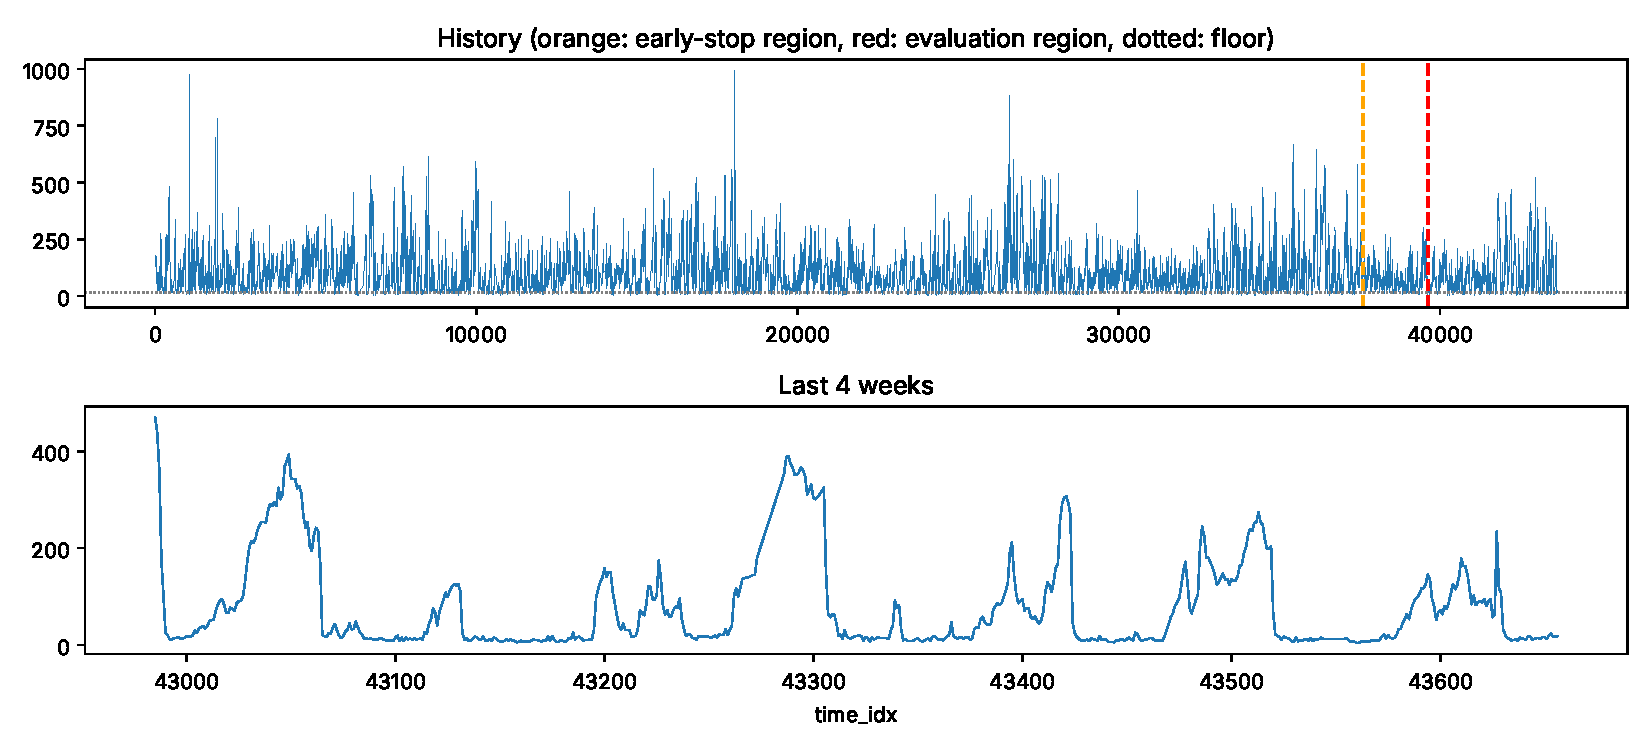
\includegraphics[width=0.95\linewidth]{figures/t2-series.pdf}
\caption{Task 2 history with the early-stop (orange) and evaluation (red) regions; the dotted line is the forecast floor (14.7).}
\label{fig:t2series}
\end{figure}

\begin{figure}[H]\centering
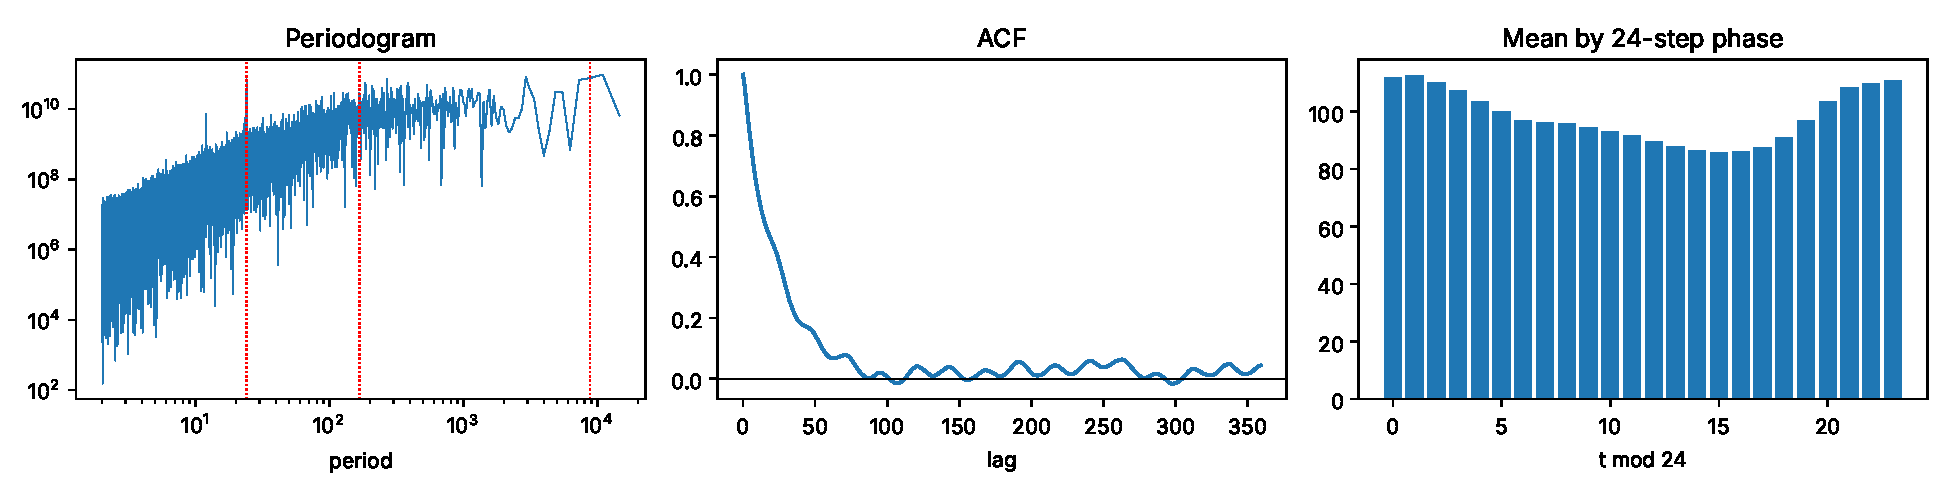
\includegraphics[width=\linewidth]{figures/t2-periodicity.pdf}
\caption{Periodogram, autocorrelation and mean by 24-step phase.}
\label{fig:t2period}
\end{figure}

\begin{itemize}
  \item \textbf{Recovered periods.} The periodogram peaks at \textbf{24} steps and near \textbf{8{,}730} ($\approx$8{,}766), so the sampling interval is most likely hourly, with daily and yearly cycles. The daily cycle is weak: the mean by phase only ranges from 86 to 113 around a mean of 98. Because no calendar is given, I encode these two measured periods as sin/cos ``phase'' features in place of Autoformer's time stamps.
  \item \textbf{Short memory.} The ACF is 0.97 at lag 1, 0.40 at lag 24, 0.16 at lag 48 and 0.03 at lag 168. The recent past says little about most of a 168-step horizon.
  \item \textbf{Heavy tails.} Values range from 0 to 994 and change by an order of magnitude within days. Exact zeros are essentially absent (2 of 43{,}656 hours).
  \item \textbf{External file.} Six continuous features (A--F) and four mutually exclusive flags (G--J). Level correlations with the target are weak (D $-0.25$, H $-0.21$, A $+0.17$, J $+0.15$) and first-difference correlations are near zero, so whether they help had to be settled experimentally. I apply \texttt{log1p} to the heavy-tailed counters D--F, standardise the continuous features on the training region, and keep the flags as 0/1.
\end{itemize}

% ---------------------------------------------------------------------
\subsection*{Validation protocol}

\begin{itemize}
  \item \textbf{Chronological split:} train on steps 1--37{,}608; early stopping only on the next 12 weeks (37{,}609--39{,}624); evaluation on the final \textbf{24 non-overlapping 168-step weeks} (39{,}625--43{,}656), which are never used for fitting or stopping.
  \item \textbf{Metrics:} MAE, RMSE and sMAPE are computed per 168-step week (one leaderboard-sized score each) and averaged over weeks. Weeks 12--23 are the most recent and most volatile, and serve as the closest analogue of the leaderboard week.
  \item \textbf{Seeds:} every configuration uses 3 seeds and is reported as mean $\pm$ std. Differences between configurations are also tested per week (paired, with a 95\% CI over the 24 weeks).
\end{itemize}

\begin{table}[H]\centering\small
\caption{Naive baselines on the 24 evaluation weeks.}
\label{tab:t2base}
\begin{tabular}{lccc}
\toprule
Baseline & MAE & RMSE & sMAPE (\%)\\
\midrule
Persistence (last value) & 96.7 & 117.4 & 89.1\\
Seasonal naive (repeat last 24) & 85.5 & 108.2 & 95.3\\
Mean of last 168 & 68.5 & 83.2 & 80.0\\
Training mean (flat line) & 69.0 & 82.9 & 81.0\\
\bottomrule
\end{tabular}
\end{table}
\noindent Over 168 steps a flat line beats persistence by 34 RMSE, which is consistent with the short memory above. Any model has to beat $\approx$83.

% ---------------------------------------------------------------------
\subsection*{Model design}

\begin{itemize}
  \item \textbf{Autoformer body.} The Auto-Correlation and series-decomposition layers are taken from the official implementation (\href{https://github.com/thuml/Autoformer}{thuml/Autoformer}, MIT licence; Wu et al., 2021), and I wire them as in its reference model: input decomposition (moving average, kernel 25); a decoder trend initialised from the window mean and a seasonal part from zeros; Auto-Correlation in the encoder and in both decoder attentions, keeping $k=\lfloor \ln L\rfloor = 5$ delays; decomposition after every attention and feed-forward block, with the trend accumulated through the decoder.
  \item \textbf{Size:} $d_{\text{model}}=32$, 4 heads, 1 encoder and 1 decoder layer, $d_{ff}=64$. Input length 168, label length 48, \texttt{pred\_len} 168.
  \item \textbf{Embedding (my own):} a circular-conv value embedding plus a linear map of the marks (phase features + covariates), with no positional encoding. The encoder and decoder take separate marks, which is what the external-data ablation varies.
  \item \textbf{Exogenous head:} a term added at each forecast step, computed from the decoder marks over the horizon. Auto-Correlation aggregates time-shifted copies of the whole sequence, which blurs an effect tied to one step, and the head keeps that effect local. It is a 5-step convolution, a GELU and a 1$\times$1 convolution (1{,}153 parameters), so it reacts to \emph{changes} in the covariates, not only their levels.
  \item \textbf{Floor layer:} the last operation is $\max(\hat y, f)$ with $f=14.7$, the 10th percentile of the training target. It has no parameters (see below).
  \item \textbf{Training:} MSE on the standardised target; AdamW (weight decay $10^{-4}$, learning rate $3\times10^{-4}$, $3\times10^{-3}$ for the head); cosine schedule; dropout 0.25; batch 64; training windows every 2 steps; early stopping with patience 4 (maximum 15 epochs).
\end{itemize}
Per model: \textbf{23{,}362} trainable parameters (22{,}209 body and embeddings + 1{,}153 head + 0 floor).

% ---------------------------------------------------------------------
\subsection*{External-data ablation (final model, 3 seeds)}

\begin{table}[H]\centering\small
\caption{With vs.\ without the optional file: mean $\pm$ std over 3 seeds, 24 evaluation weeks.}
\label{tab:t2abl}
\begin{tabular}{lccc}
\toprule
Configuration & MAE & RMSE & sMAPE (\%)\\
\midrule
Target only & 68.2 $\pm$ 2.2 & 82.5 $\pm$ 1.7 & 78.9 $\pm$ 0.9\\
+ external (past only, encoder) & 68.9 $\pm$ 2.4 & 82.8 $\pm$ 1.4 & 79.4 $\pm$ 1.1\\
+ external (past + horizon, encoder and decoder) & \textbf{42.0 $\pm$ 2.4} & \textbf{56.8 $\pm$ 3.0} & \textbf{52.0 $\pm$ 0.3}\\
\bottomrule
\end{tabular}
\end{table}

\begin{figure}[H]\centering
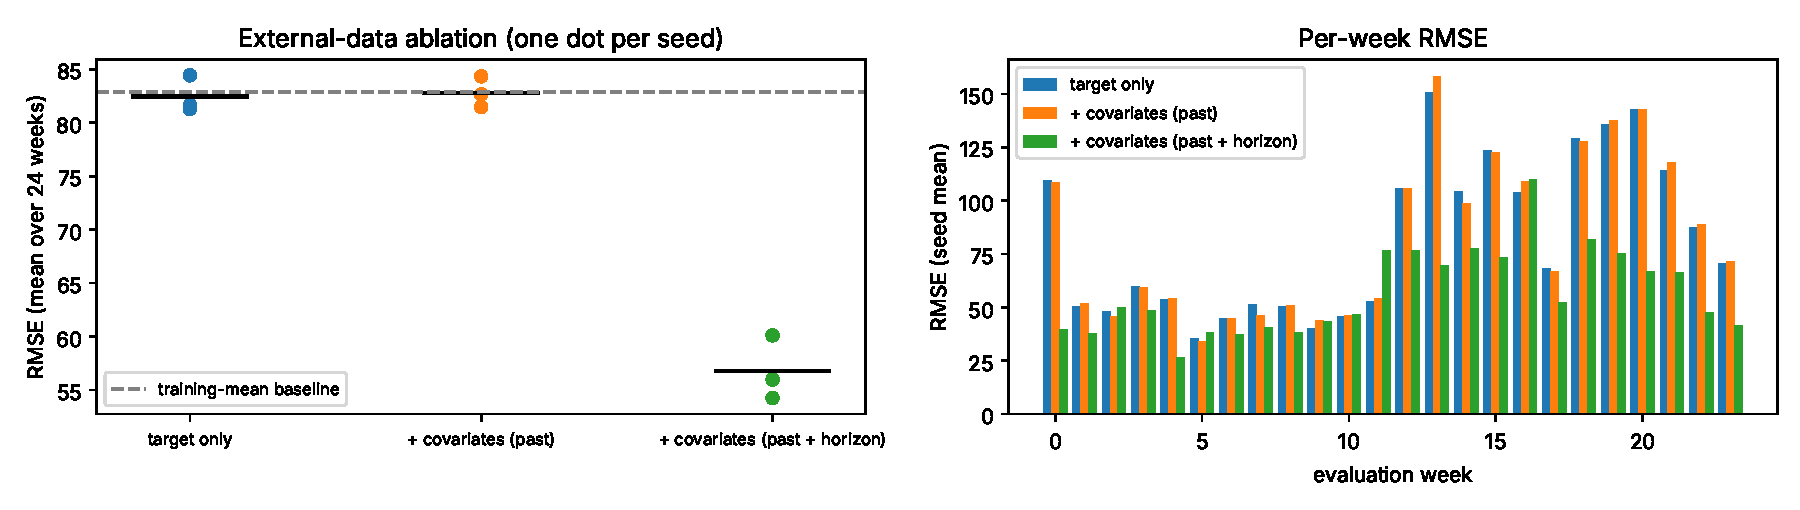
\includegraphics[width=\linewidth]{figures/t2-ablation.pdf}
\caption{External-data ablation: RMSE per seed (left) and per evaluation week (right).}
\label{fig:t2abl}
\end{figure}

\begin{itemize}
  \item \textbf{Covariates help only when they cover the horizon.} Past + horizon vs.\ target only: $\Delta$RMSE $=-25.7 \pm 11.3$, better on 18/24 weeks. Past only vs.\ target only: $+0.4 \pm 1.2$, better on 10/24, i.e.\ no effect.
  \item \textbf{Interpretation.} The covariates are measured on the same clock as the target and are known over the forecast window. Knowing them up to the forecast origin adds nothing, because the target's own memory is short. Their value lies in describing conditions \emph{during} the horizon, so they must enter the decoder.
  \item Without the horizon covariates, the Autoformer is no better than a flat line (82.5 vs.\ 82.9).
\end{itemize}

% ---------------------------------------------------------------------
\subsection*{Submissions and design changes}

Each change below was decided on the evaluation weeks before submitting; the leaderboard was used only to confirm.

\begin{table}[H]\centering\small
\caption{The three leaderboard submissions. Validation = RMSE over the 24 evaluation weeks (all / weeks 12--23) of exactly the configuration submitted.}
\label{tab:t2subs}
\begin{tabular}{clccccc}
\toprule
\# & Model & Val.\ all & Val.\ 12--23 & $P$ & $E$ & Leaderboard RMSE (rank)\\
\midrule
1 & Linear head, 1 seed, no refit, clip at 0 & 63.8 & 79.3 & 22{,}224 & 4 & 93.82 ($\sim$23rd)\\
2 & Non-linear head, 3 seeds + refit, floor after prediction & 56.0 & 71.4 & 70{,}086 & 18 & 71.48 (8th)\\
3 & Non-linear head, 3 seeds + refit, \textbf{floor layer} & \textbf{54.3} & \textbf{68.3} & 70{,}086 & 18 & \textbf{67.22 (3rd)}\\
\bottomrule
\end{tabular}
\end{table}

\begin{table}[H]\centering\small
\caption{Design checks on the past + horizon configuration (3 seeds, RMSE mean $\pm$ std over seeds).}
\label{tab:t2design}
\begin{tabular}{lcc}
\toprule
Configuration & All 24 weeks & Weeks 12--23\\
\midrule
Linear head, dropout 0.1, LR halved each epoch (submission 1) & 60.50 $\pm$ 2.48 & 75.87 $\pm$ 2.43\\
Linear head, dropout 0.25, weight decay, cosine LR & 61.17 $\pm$ 2.11 & 76.20 $\pm$ 2.46\\
Non-linear head, clipped at 0 & 58.12 $\pm$ 2.37 & 72.72 $\pm$ 2.40\\
Non-linear head, floored after prediction (submission 2) & 57.85 $\pm$ 2.42 & 72.58 $\pm$ 2.43\\
Non-linear head, floor layer (submission 3) & \textbf{56.77 $\pm$ 2.46} & \textbf{69.89 $\pm$ 2.37}\\
\midrule
Linear head + 12 more recent weeks in training (refit check) & 59.97 $\pm$ 2.39 & 75.16 $\pm$ 2.37\\
\bottomrule
\end{tabular}
\end{table}

\begin{itemize}
  \item \textbf{Submission 1} scored 93.8 against a validation mean of 60.5. The calm early weeks had flattered the average: on the recent weeks the same model scored 79.3, with weekly RMSE ranging from 33 to 101. From then on I selected on weeks 12--23.
  \item \textbf{Regularisation did not help} ($+0.67 \pm 1.36$, better on 6/24 weeks). Every run still peaked at epoch 1 or 2, so the early stop was not driven by memorisation. Training and recent periods differ, and the covariate head learns the simple signal within one epoch.
  \item \textbf{Non-linear covariate head:} $-3.05 \pm 4.41$ vs.\ the linear head, better on 17/24 weeks. The large errors occur at sudden changes, which a 5-step convolution can represent.
  \item \textbf{Refit and seed averaging.} Training on 12 more recent weeks improved every seed ($-0.53$ RMSE), so the final models are refit on the full history. Averaging the 3 seeds lowers RMSE by a further 1.5--2.5.
  \item \textbf{Floor layer:} $-1.08 \pm 2.63$ RMSE vs.\ the post-hoc floor, but $-3.1$ on the seed-averaged recent weeks (71.40 $\to$ 68.34), and MAE 45.7 $\to$ 42.0.
  \item \textbf{Calibration.} The recent-week validation estimate predicted submissions 2 and 3 to within about one point (71.4 vs.\ 71.48; 68.3 vs.\ 67.22). Submission~1's larger gap is explained by having selected on all 24 weeks.
\end{itemize}

% ---------------------------------------------------------------------
\subsection*{The forecast floor}

\begin{itemize}
  \item \textbf{Why a floor.} The target is non-negative and effectively never zero. Clipping negative outputs at 0 (submission 1) produced runs of exact zeros, whereas on validation weeks where the raw output was negative the truth averaged 14. I therefore use the 10th percentile of the training target, 14.7, fixed from training data only. This is post-hoc truncation to the plausible range; a log or scaled-logit transform (Hyndman \& Athanasopoulos, FPP3 \S13.3) would build the constraint into the model instead.
  \item \textbf{After prediction vs.\ inside the network.} The same $\max(\hat y, 14.7)$ gives different forecasts. Applied after prediction (submission 2), it trims a model that was trained without it and had learned realistic low values (raw outputs mostly between $-20$ and 50 in the low periods of this forecast). Applied as a layer during training (submission 3), it changes what the model learns. The two submissions differ by 18 RMSE.
  \item \textbf{Repeated values of 14.70.} The final forecast sits exactly at 14.70 for 44 of 168 hours (the first 16 and the last 26). In these hours the covariates show the pattern that historically means low values (high C, accumulating D, flag H; hours with this pattern averaged 23, median 16), and all three seeds are clamped. Underneath, the raw outputs are $-35$ to $-390$: because $\partial \max(\hat y, f)/\partial \hat y = 0$ below the floor, no gradient pulls them back, so the model can only say ``at the floor''. This is a limitation, although validation favours it, and a flat 14.70 everywhere would be far worse (RMSE 104.5).
  \item \textbf{Why $P$ and $E$ are identical for submissions 2 and 3.} The floor layer stores 14.7 as a constant, not a trainable weight, so both use $3 \times 23{,}362 = 70{,}086$ parameters. In both, every seed's best early-stopping epoch was 1, with 5 epochs run, giving $E = 3 \times (5 + 1) = 18$.
  \item \textbf{The floor could also be learned.} A learnable floor level (1 parameter per model) would let training choose the level instead of the 10th-percentile rule. A smooth floor ($f + \mathrm{softplus}(\hat y - f)$) would keep a gradient below the floor, so the model could predict, say, 18 or 25 in low periods instead of a flat 14.70. I left both untested: the expected gain was small, the last submission replaces the score, and submission~3 already matched its validation estimate. They are the first next step.
\end{itemize}

% ---------------------------------------------------------------------
\subsection*{Final model: validation and forecast}

\begin{table}[H]\centering\small
\caption{Final model on the 24 evaluation weeks.}
\label{tab:t2final}
\begin{tabular}{lcccccc}
\toprule
Seed & MAE & RMSE & sMAPE (\%) & RMSE weeks 12--23 & Best epoch & Epochs run\\
\midrule
0 & 44.52 & 60.10 & 51.74 & 72.89 & 1 & 5\\
1 & 41.63 & 55.98 & 51.93 & 69.72 & 1 & 5\\
2 & 39.80 & 54.24 & 52.28 & 67.08 & 1 & 5\\
\textbf{3-seed average} & \textbf{40.01} & \textbf{54.26} & \textbf{49.32} & \textbf{68.34} & -- & --\\
\bottomrule
\end{tabular}
\end{table}

\begin{figure}[H]\centering
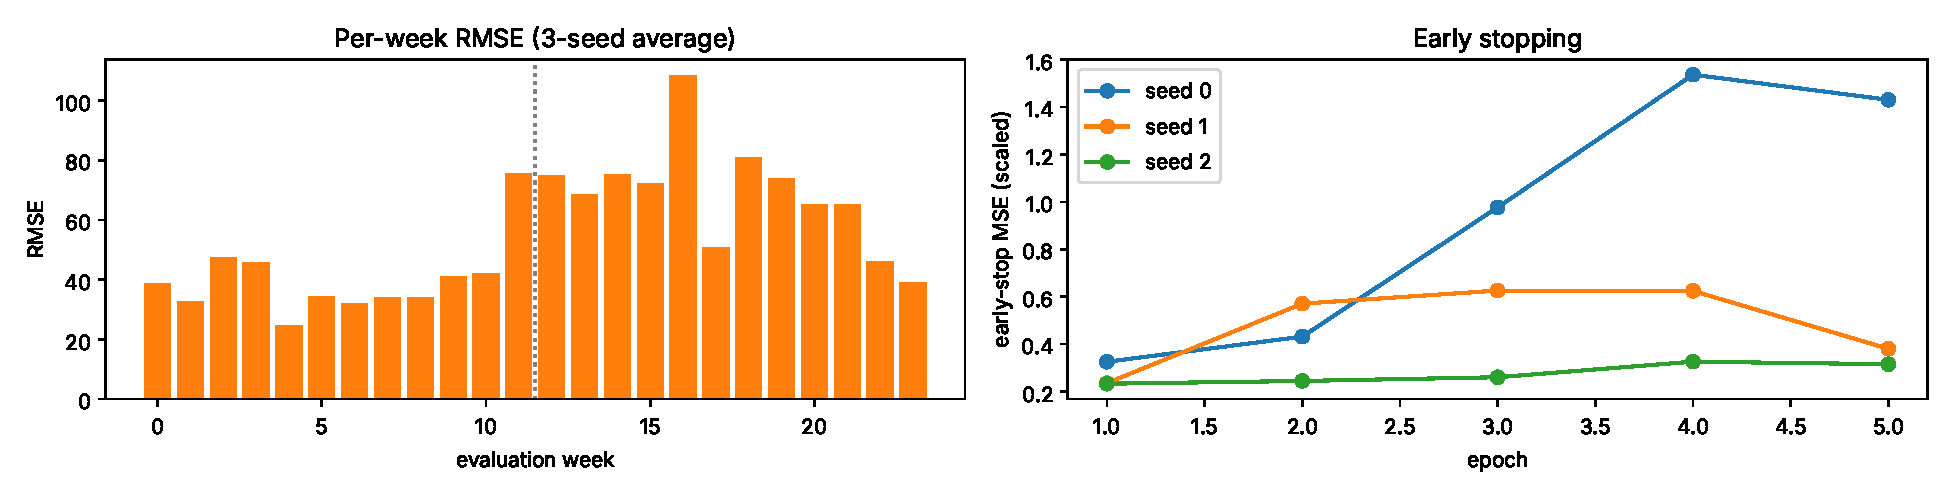
\includegraphics[width=\linewidth]{figures/t2-validation.pdf}
\caption{Final model: per-week RMSE of the 3-seed average (left); early-stopping loss per seed (right).}
\label{fig:t2val}
\end{figure}

\begin{figure}[H]\centering
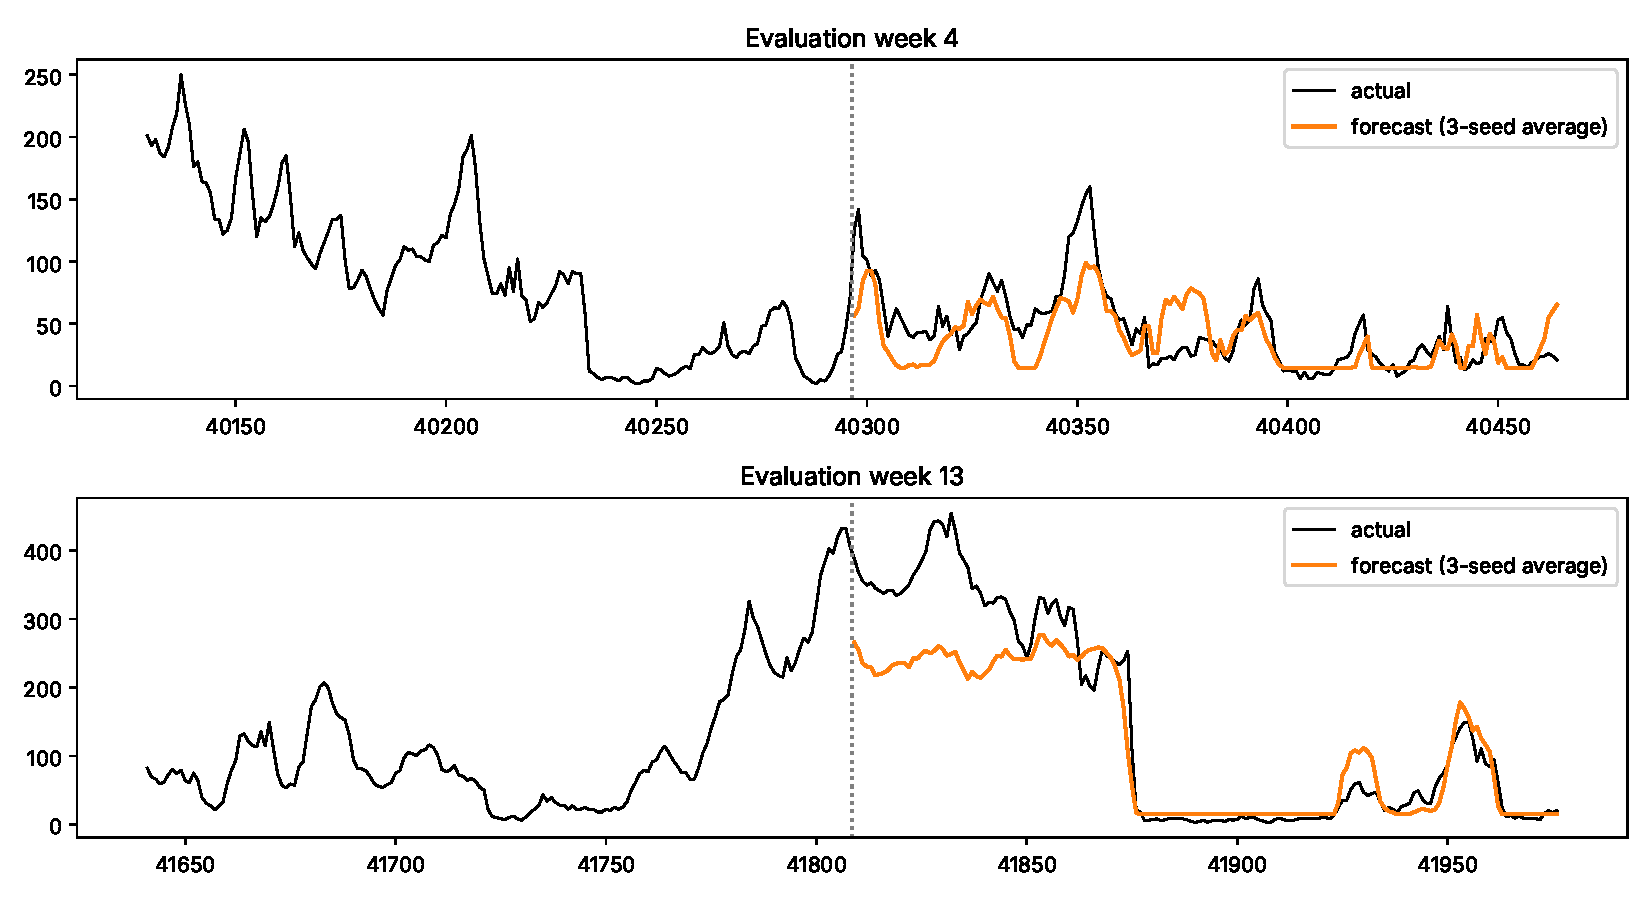
\includegraphics[width=0.95\linewidth]{figures/t2-example-weeks.pdf}
\caption{Two evaluation weeks: actual vs.\ the 3-seed average forecast.}
\label{fig:t2weeks}
\end{figure}

\begin{figure}[H]\centering
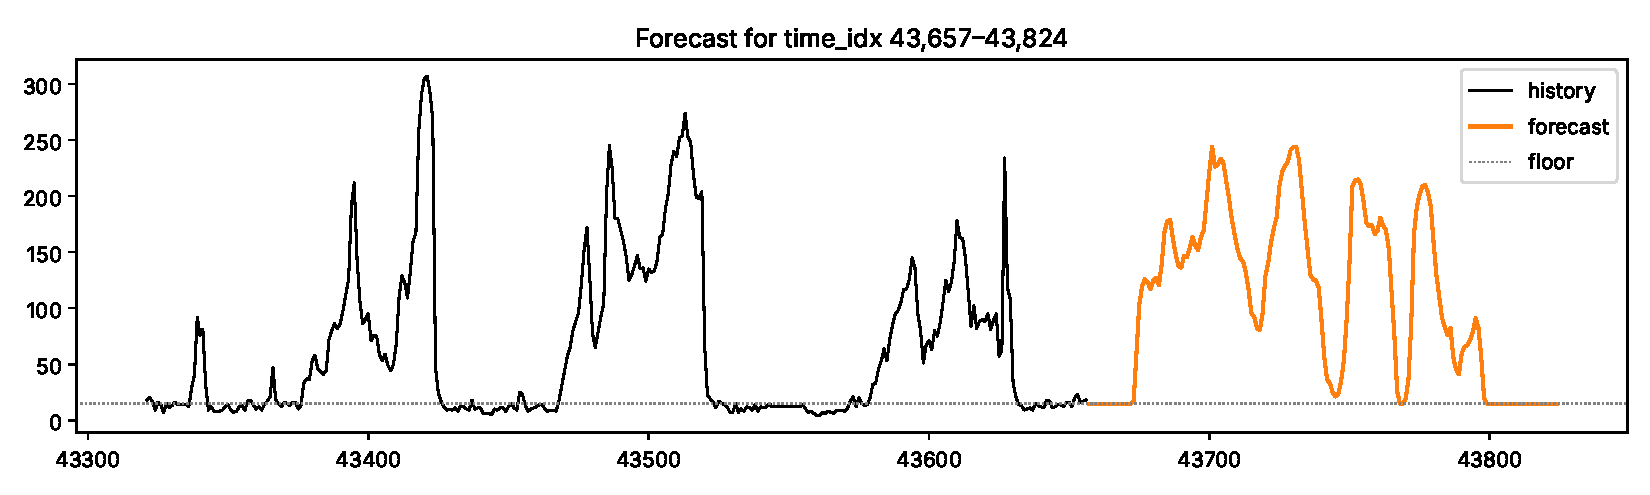
\includegraphics[width=0.95\linewidth]{figures/t2-forecast.pdf}
\caption{Submitted forecast for \texttt{time\_idx} 43{,}657--43{,}824.}
\label{fig:t2fc}
\end{figure}

\begin{infobox}{Final submission (third attempt)}
Each seed is refit on all 43{,}656 steps for its early-stopped epoch count (1), and the three forecasts are averaged.
$P = 3 \times 23{,}362 = \mathbf{70{,}086}$; $E = \sum_{\text{seeds}}(\text{early-stopping epochs run} + \text{refit epochs}) = 3 \times (5+1) = \mathbf{18}$.
Leaderboard: MAE 46.22, \textbf{RMSE 67.22}, sMAPE 42.79\%, score 67.225, \textbf{rank 3}.
\end{infobox}

\paragraph{Limitations.} Early stopping chose epoch 1 in every run, so the Autoformer body adds less than its size suggests; the covariate head carries much of the gain, consistent with Zeng et al.\ (2023). A plain ridge regression on the horizon covariates reached RMSE 57.3 on the same weeks, close to the final model's 54.3.
